% LaTeX Beamer From Scratch
%%
% Andre Pereira andrespp at gmail dot com
% 13/10/2009
%
% This document is based on the Beamer User Guide, available at:
% http://www.ctan.org/tex-archive/macros/latex/contrib/beamer/doc/beameruserguide.pdf

\documentclass{beamer}

%%%Style setup
%\usetheme{Madrid} 	% Very clean
%\usetheme{Antibes}	% 3 top bars: section, subsection, subsubsection
\usetheme{Frankfurt}	% 2 top bars: section, slide counter %%esse
%\usetheme{Ilmenau}
%\usetheme{Berlin}	% 2 top bars: section, slide counter
%\usetheme{Warsaw}	% large top bar
%\usetheme{Bergen} 	% left side bar (uhhg)
%\usetheme{Rochester} 	% clean with large top bar
%\usetheme{Darmstadt}
%\usetheme{Boadilla}	% super clean
%\usetheme{Copenhagen}
%\usetheme{Dresden}	% 2 top bars
%\usetheme{Malmoe}
%\usetheme{Goettingen}	% clear right bar
%\usetheme{Hannover}	% clear left bar
%\usetheme{Ilmenau}
%\usetheme{JuanLesPins}	% 3 top bars (slim)
%\usetheme{Luebeck}
%\usetheme{Marburg}	% bold right bar
%\usetheme{PaloAlto}	% left / top bar
%\usetheme{Singapore}	% clear top bar
%\usetheme{Szeged}
%\usetheme{default}	% totaly white background
%\usetheme{Montpellier}

%\usecolortheme{seahorse}	%diminui o contraste
%\usecolortheme{rose}			%diminui o contraste
%\usefonttheme[onlylarge]{structuresmallcapsserif}

% Hide slide bullets on header
\setbeamertemplate{headline}
 {%
  \begin{beamercolorbox}{section in head/foot}
  \insertsectionnavigationhorizontal{\textwidth}{}{}
  \end{beamercolorbox}%
}


%%%Package Setup
\usepackage[brazil]{babel}
\usepackage[utf8]{inputenc} 	%uso de acentos - linux
%\usepackage[latin1]{inputenc} %uso de acentos - windows
\usepackage{listings}
\usepackage{subfig}

%%%Document Setup
\mode<presentation>
\title{\textit{Scheduling of Domestic Shiftable Loads via Cuckoo Search
Optimization Algorithm}}
%\subtitle{Trabalho da Disciplina PPGEE0248 - Tópicos Especiais em Computação
%Aplicada}
%\author{André Augusto da Silva Pereira\\ andresp@las.ic.unicamp.br}
\author{André Pereira \\
	Daniel Victor \\
        Junior Albuquerque \\
        Sandio Maciel \\
        Thiago Ferreira \\
}
%			\textbf{Professor:} Prof. Dr. Paulo Lício de Geus}

\date{Novembro/2018}
\institute{Universidade Federal do Pará \\
Programa de Pós-Graduação em Engenharia Elétrica}

%%%Document itself
\begin{document}
%	\def\newblock{\hskip .11em plus .33em minus .07em} %bibliography fix
  \setbeamertemplate{footline}[frame number]
  \pgfdeclareimage[height=0.95cm] {logo}{./Figures/ufpa}
	\logo{\pgfuseimage{logo}}

\begin{frame}
  \titlepage
\end{frame}

\begin{frame}
  \begin{figure}[h]
  	\begin{center}
      
\includegraphics [scale=0.23]{./Figures/article}
     % \caption {Estimativa de dispositivos conectados à Internet.}
  		%\label{fig:arq-imuno}
  	\end{center}
  \end{figure}
\end{frame}

\begin{frame}{Agenda}
	\tableofcontents
\end{frame}

\section{Introdução}

\frame{\tableofcontents[currentsection]}

\begin{frame}{\textit{Redes de Distribuição}}
  \begin{block}{Modelo Tradicional}
    \begin{itemize}
      \item Grandes geradoras de energia, geralmente próximas às fontes
      primárias de energica
      \item Energia produzida e transmitida aos grandes centros, para então ser
      distribuída aos consumidores
    \end{itemize}
  \end{block}
  \begin{figure}[h]
  	\begin{center}
      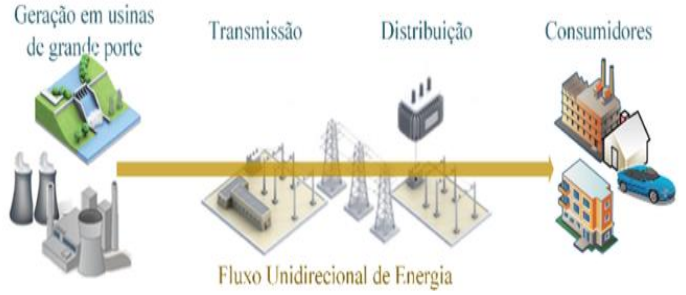
\includegraphics [scale=0.333]{./Figures/TraditionalGrid}
      %\caption {Valores da Tarifa Branca - CELPA (Fonte:}
  		%\label{fig:arq-imuno}
  	\end{center}
  \end{figure}
\end{frame}

\begin{frame}{Redes de Distribuição}
  \begin{block}{Modelo de Rede Inteligente - \textbf{\textit{Smart Grid}}}
    \begin{itemize}
      \item Integração de \alert{TIC} para fins de monitoramento e tráfego de
      informações
      \item Alto grau de \alert{automação} da rede de distribuição
      (confiabilidade/flexibilidade)
      \item \alert{Interação do consumidor} com a rede de distribuição:
      \begin{itemize}
        \item Ciente e participativo com relação ao consumo
        \item Gerenciamento pelo lado da demanda
        \item Geração de energia pelo lado da demanda (geração distribuída)
      \end{itemize}
    \end{itemize}
  \end{block}
  \begin{figure}[h]
  	\begin{center}
      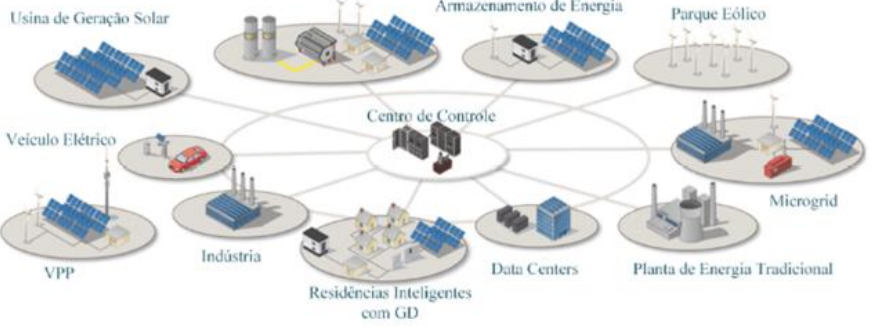
\includegraphics [scale=0.27]{./Figures/SmartGrid}
      %\caption {Valores da Tarifa Branca - CELPA (Fonte:}
  		%\label{fig:arq-imuno}
  	\end{center}
  \end{figure}
\end{frame}

\begin{frame}
  \begin{block}{Gerenciamento pelo lado da Demanda}
    \begin{itemize}
      \item Modifica perfil de consumo através de incentivos financeiros
      \item Busca um consumo de acordo com o perfil desejado, e não uma geração
      de acordo com a demanda
      \item Diversas técnicas propostas na literatura:
      \begin{itemize}
        \item Preços dinâmicos (ex: Tarifa Branca)
        \item Controle e escalonamento da utilização de equipamentos pela
        distribuidora
      \end{itemize}
    \end{itemize}
  \end{block}
\end{frame}

\begin{frame}
  \begin{figure}[h]
  	\begin{center}
      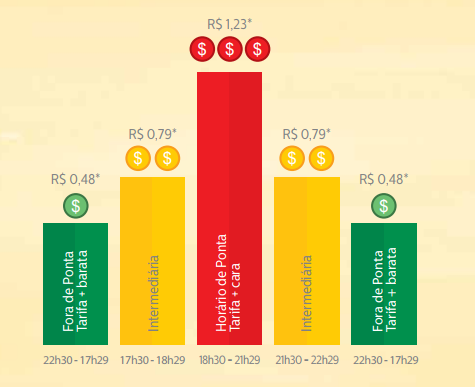
\includegraphics [scale=0.7]{./Figures/TarifaBranca}
      \caption {Valores da Tarifa Branca - CELPA (Fonte:
      http://www.celpa.com.br/imobiliario/simuladores/consumo-de-energia-na-tarifa-branca).}
  		%\label{fig:arq-imuno}
  	\end{center}
  \end{figure}
\end{frame}

\begin{frame}
  \begin{block}{Consumo doméstico}
    \begin{itemize}
      \item Utensílios domésticos possuem alto consumo:
      \begin{itemize}
        \item Lava louças, lava roupas, secadora, etc ...
      \end{itemize}
      \item Podem sobrecarregar a rede em caso de uso simultâneo
      \item Controle sobre o escalonamento destes equipamentos podem evitar
      as sobrecargas
    \end{itemize}
  \end{block}
  \pause
  \begin{block}{Algoritmos de Escalonamento propostos na Literatura}
    \begin{itemize}
      \item Abordagens:
      \begin{itemize}
        \item \textit{Particle Swarm Optimization} (PSO)
        \item Altoritmos evolucionários (GA)
        \item \textit{Cuckoo Search algorithm} (CSA)
      \end{itemize}
    \end{itemize}
  \end{block}
\end{frame}

\begin{frame}
  Neste trabalho, cargas domésticas são escalonados pelo CSA visando o
  balanceamento da curva de carga da rede, levando em consideração as o máximo
  possível as preferências dos usuários
  \begin{block}{Considerações}
    \begin{itemize}
      \item Agendamento considera a carga do transformador, e não da residência
      \item 4 consumidores
      \item 5 cargas comutáveis por consumidor
      \item Algoritmo de escalonamento ótimo baseado em CSA
      \item Resultados comparados com otimizador baseado em AG
    \end{itemize}
  \end{block}
\end{frame}

%\begin{frame}
%  \begin{block}{}
%    \begin{itemize}
%      \item
%    \end{itemize}
%  \end{block}
%\end{frame}

%\begin{frame}
%  \begin{block}{}
%  \end{block}
%\end{frame}

%\begin{frame}
%  \begin{figure}[h]
%  	\begin{center}
%      \includegraphics [scale=0.3]{./Figures/Device-Estimates}
%     % \caption {Estimativa de dispositivos conectados à Internet.}
%  		%\label{fig:arq-imuno}
%  	\end{center}
%  \end{figure}
%\end{frame}

%\begin{frame}{Redes de Acesso}
%	\begin{figure}[!htb]
%		\centering
%		\subfloat[DSL]{
%			\includegraphics[height=3.5cm]{./Figures/DSLaccess}
%			\label{figdroopy}}
%		\quad %espaco separador
%		\subfloat[Cable]{
%			\includegraphics[height=3.5cm]{./Figures/CableAccess}
%			\label{figsnoop}}
%		%\caption{Subfiguras}
%		%\label{fig01}
%	\end{figure}
%\end{frame}

%\begin{frame}[fragile]
%\scriptsize
%\begin{verbatim}
%\end{verbatim}
%\end{frame}

%\begin{frame}{\textit{Socket Programming with TCP}}
%\scriptsize
%\lstinputlisting[language=Python, caption={TCP Server.}]{./code/upperServer/TCPserver.py}
%\end{frame}


\section[Appliances]{Escalonamento e Gerenciamento de Utensílios Domésticos}
\frame{\tableofcontents[currentsection]}
\begin{frame}
  \begin{block}{Tipos de utensílios domésticos}
    \begin{itemize}
      \item Eletrodomésticos podem ser divididos em três grupos:
      \begin{itemize}
        \item \textbf{Agendáveis:} Lava-louças, lava-roupas, ...
        \item \textbf{Reguláveis:} Ar-condicionado, aquecedor, ...
        \item \textbf{Essenciais:} TVs, fornos elétricos, lâmpadas, ...
      \end{itemize}
    \end{itemize}
  \end{block}
  \pause
  \begin{block}{Perfil de operação}
    \begin{itemize}
      \item Possuem características/restrições de período de utilização:
      \begin{itemize}
        \item \textbf{Agendáveis:} operação pode ser agendada/escalonada
        \item \textbf{Reguláveis:} tendem a ser utilizados em períodos fixos
        \item \textbf{Essenciais:} são utilizados em períodos específicos
        e demandam energia constante
      \end{itemize}
    \end{itemize}
  \end{block}
\end{frame}

\begin{frame}
  \begin{block}{Possíveis abordagens em \textit{Smart Grids}}
    \begin{itemize}
      \item Em uma rede inteligente, para cada grupo pode-se:
      \begin{itemize}
        \item \textbf{Agendáveis:} operadora pode agendar utilização para
        horários fora de pico, através de políticas preço (preço é um icentivo,
        mas conforto deve ser levado em consideração)
        \item \textbf{Reguláveis:} operadora pode otimizar parâmetros de
        utilização/consumo, sem contudo mudar o horário de funcionamento
        \item \textbf{Essenciais:} operadora não pode interferir na utilização,
        contudo pode prever a demanda diária e planejar a utilização da rede
        para garantir o balanço geração \textit{vs} consumo
      \end{itemize}
    \end{itemize}
  \end{block}
\end{frame}

%\begin{frame}
%  \begin{block}{}
%    \begin{itemize}
%      \item
%    \end{itemize}
%  \end{block}
%\end{frame}

%\begin{frame}
%  \begin{block}{}
%  \end{block}
%\end{frame}

%\begin{frame}
%  \begin{figure}[h]
%  	\begin{center}
%      \includegraphics [scale=0.3]{./Figures/Device-Estimates}
%     % \caption {Estimativa de dispositivos conectados à Internet.}
%  		%\label{fig:arq-imuno}
%  	\end{center}
%  \end{figure}
%\end{frame}

%\begin{frame}{Redes de Acesso}
%	\begin{figure}[!htb]
%		\centering
%		\subfloat[DSL]{
%			\includegraphics[height=3.5cm]{./Figures/DSLaccess}
%			\label{figdroopy}}
%		\quad %espaco separador
%		\subfloat[Cable]{
%			\includegraphics[height=3.5cm]{./Figures/CableAccess}
%			\label{figsnoop}}
%		%\caption{Subfiguras}
%		%\label{fig01}
%	\end{figure}
%\end{frame}

%\begin{frame}[fragile]
%\scriptsize
%\begin{verbatim}
%\end{verbatim}
%\end{frame}

%\begin{frame}{\textit{Socket Programming with TCP}}
%\scriptsize
%\lstinputlisting[language=Python, caption={TCP Server.}]{./code/upperServer/TCPserver.py}
%\end{frame}



\section[Algoritmo]{Algoritmo Proposto}
\frame{\tableofcontents[currentsection]}
\begin{frame}
  \begin{block}{Algoritmo de Escalonamento de Cargas domésticas baseado em CSA}
    \begin{itemize}
      \item O \textit{Cucko Search Algorithm} (CSA) é um algoritmo
      metaheurístico
      \item ...
    \end{itemize}
  \end{block}
  \begin{figure}[h]
  	\begin{center}
      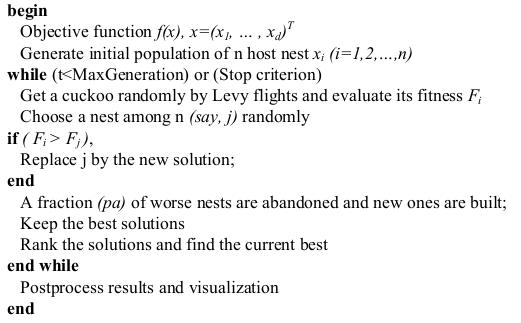
\includegraphics [scale=0.35]{./Figures/csa}
      \caption {Pseudo-código do CSA utilizando vôos de Levy.}
  		%\label{fig:arq-imuno}
  	\end{center}
  \end{figure}
\end{frame}

\begin{frame}
  \begin{block}{}
    \begin{itemize}
      \item Este trabalho é utilizado para determinar o horário de inicio de
      utilização de \alert{utensílios agendáveis}
      \begin{itemize}
        \item Inicialmente obtem-se as preferências dos clientes
        \item Em seguida obtem-se a curva de consumo desejada para a rede
        \item Finalmente o CSA é utilizado para obter-se os horários ótimos de
        inicio de opearação
      \end{itemize}
    \end{itemize}
  \end{block}
  \begin{figure}[h]
  	\begin{center}
      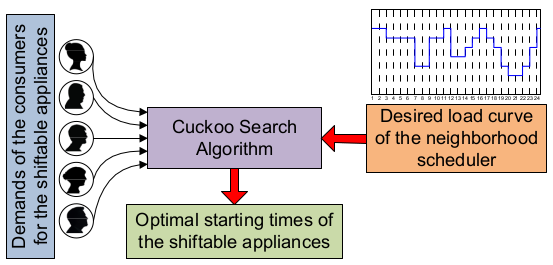
\includegraphics [scale=0.35]{./Figures/CSscheme}
      \caption {Diagrama de blocos da solução proposta.}
  		%\label{fig:arq-imuno}
  	\end{center}
  \end{figure}
\end{frame}

%\begin{frame}
%  \begin{block}{}
%    \begin{itemize}
%      \item
%    \end{itemize}
%  \end{block}
%\end{frame}

%\begin{frame}
%  \begin{block}{}
%  \end{block}
%\end{frame}

%\begin{frame}
%  \begin{figure}[h]
%  	\begin{center}
%      \includegraphics [scale=0.3]{./Figures/Device-Estimates}
%     % \caption {Estimativa de dispositivos conectados à Internet.}
%  		%\label{fig:arq-imuno}
%  	\end{center}
%  \end{figure}
%\end{frame}

%\begin{frame}{Redes de Acesso}
%	\begin{figure}[!htb]
%		\centering
%		\subfloat[DSL]{
%			\includegraphics[height=3.5cm]{./Figures/DSLaccess}
%			\label{figdroopy}}
%		\quad %espaco separador
%		\subfloat[Cable]{
%			\includegraphics[height=3.5cm]{./Figures/CableAccess}
%			\label{figsnoop}}
%		%\caption{Subfiguras}
%		%\label{fig01}
%	\end{figure}
%\end{frame}

%\begin{frame}[fragile]
%\scriptsize
%\begin{verbatim}
%\end{verbatim}
%\end{frame}

%\begin{frame}{\textit{Socket Programming with TCP}}
%\scriptsize
%\lstinputlisting[language=Python, caption={TCP Server.}]{./code/upperServer/TCPserver.py}
%\end{frame}




\section[Resultados]{Simulações e Resultados}
\frame{\tableofcontents[currentsection]}
\begin{frame}  
  \begin{figure}[h]
  	\begin{center}
      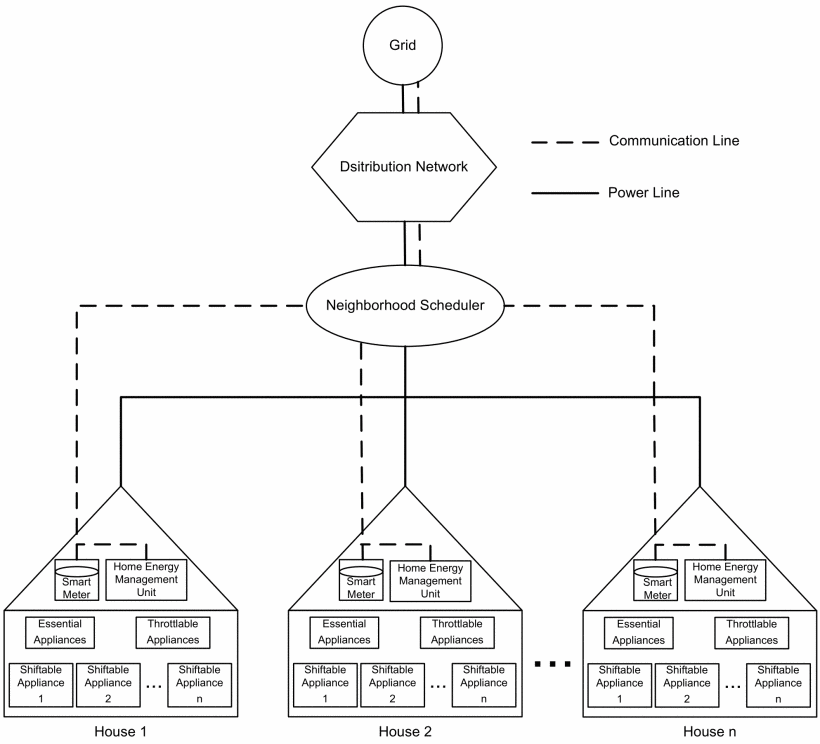
\includegraphics [scale=0.3]{./Figures/result1}
      \caption {Estrutura do sistema simulado e proposto}
  		%\label{fig:arq-imuno}
  	\end{center}
  \end{figure}
\end{frame}

\begin{frame}
  \begin{block}{}
    \begin{itemize}
      \item \alert{L1}, \alert{L2}, \alert{L3}, \alert{L4} e \alert{L5} respresentam as cargas deslocáveis dadas pelo consumidor
      \item Intervalos de demanda preferíveis informados pelo consumidor
      \item Valor ótimo gerado pelo algoritmo 
    \end{itemize}  
  \end{block}
  
  \begin{figure}[h]
  	\begin{center}
      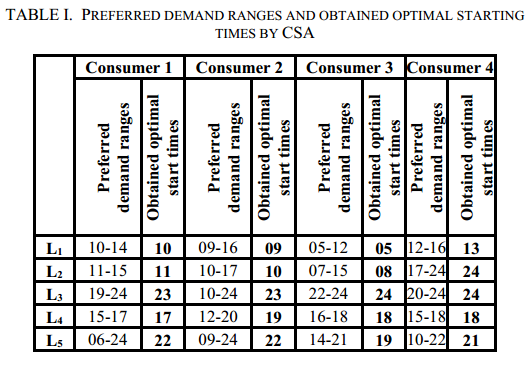
\includegraphics [scale=0.45]{./Figures/result2}
      \caption {\footnotesize Faixas de demandas preferidas pelo usuário e tempo de iniciação ótimo obtido pelo CSA}
  		%\label{fig:arq-imuno}
  	\end{center}
  \end{figure}
\end{frame}

\begin{frame}
  \begin{block}{}
    \begin{itemize}
      \item Os dados são aplicados ao \alert{AG} e ao \alert{CSA}
      \item Na figura é possível observar que o CSA se demonstrou mais eficiente que o AG (10 experimentos realizados)
      \item Melhores valores de fitness: 218.000 (AG) e 176.000 (CSA) 
    \end{itemize}
  \end{block}
  
  \begin{figure}[h]
  	\begin{center}
      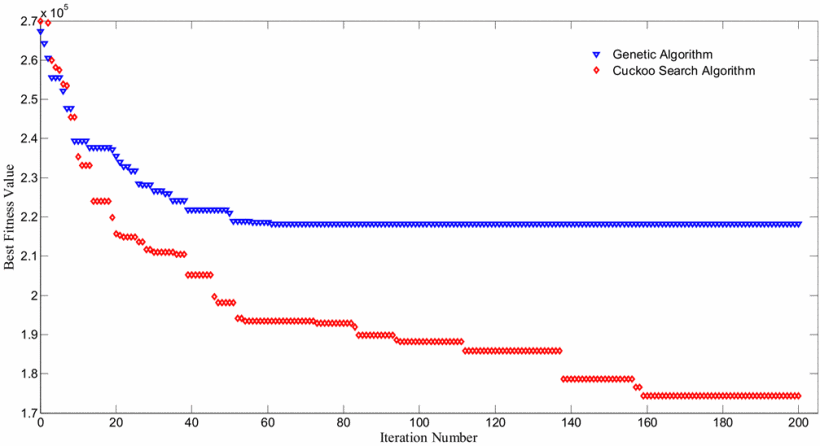
\includegraphics [scale=0.32]{./Figures/result3}
      \caption {Comparativo entre os resultados dos algoritmos de otimização}
  		%\label{fig:arq-imuno}
  	\end{center}
  \end{figure}
\end{frame}

\begin{frame}
  \begin{block}{}
    \begin{itemize}
      \item \small A redução da carga de pico é alcançada pelo escalonamento proposto
      \item \small \alert{O pico de carga é reduzido em 22\%}  
      \item \small A razão entre pico e média (PAR) diminuiu de 3,27 para 2,53 após o agendamento
    \end{itemize}
  \end{block}
  
  \begin{figure}[h]
  	\begin{center}
      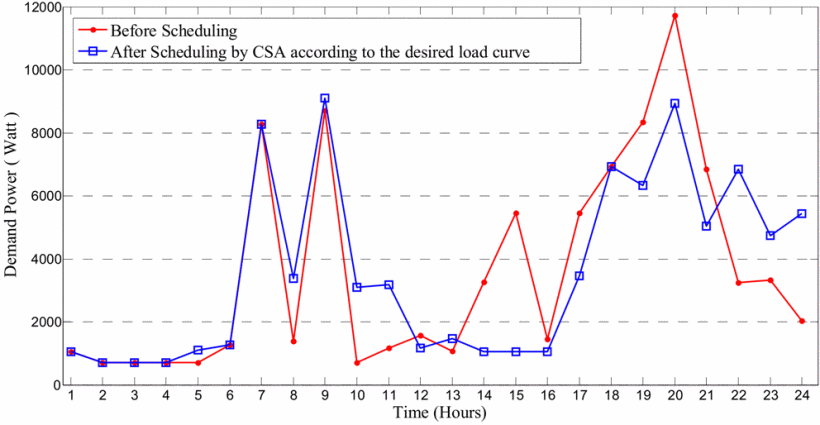
\includegraphics [scale=0.32]{./Figures/result4}
      \caption {Curvas de consumo agregado das casas}
  		%\label{fig:arq-imuno}
  	\end{center}
  \end{figure}
\end{frame}
%\begin{frame}
%  \begin{block}{}
%    \begin{itemize}
%      \item
%    \end{itemize}
%  \end{block}
%\end{frame}

%\begin{frame}
%  \begin{block}{}
%  \end{block}
%\end{frame}

%\begin{frame}
%  \begin{figure}[h]
%  	\begin{center}
%      \includegraphics [scale=0.3]{./Figures/Device-Estimates}
%     % \caption {Estimativa de dispositivos conectados à Internet.}
%  		%\label{fig:arq-imuno}
%  	\end{center}
%  \end{figure}
%\end{frame}

%\begin{frame}{Redes de Acesso}
%	\begin{figure}[!htb]
%		\centering
%		\subfloat[DSL]{
%			\includegraphics[height=3.5cm]{./Figures/DSLaccess}
%			\label{figdroopy}}
%		\quad %espaco separador
%		\subfloat[Cable]{
%			\includegraphics[height=3.5cm]{./Figures/CableAccess}
%			\label{figsnoop}}
%		%\caption{Subfiguras}
%		%\label{fig01}
%	\end{figure}
%\end{frame}

%\begin{frame}[fragile]
%\scriptsize
%\begin{verbatim}
%\end{verbatim}
%\end{frame}

%\begin{frame}{\textit{Socket Programming with TCP}}
%\scriptsize
%\lstinputlisting[language=Python, caption={TCP Server.}]{./code/upperServer/TCPserver.py}
%\end{frame}


\section{Conclusões}
\frame{\tableofcontents[currentsection]}
%\begin{frame}
%  \begin{block}{Considerações Finais}
%  \begin{itemize}
%    \item \small Realização de um estudo acerca do agendamento de cargas domésticas
%    \item \small Prospota de um mecanismo de escalonamento usando o CSA
%    \item \small Os resultados indicam que o CSA é mais eficiente para o escalonamento de cargas deslocáveis domésticas quando comparado ao GA
%    \item \small Os resultados indicam que o CSA é mais eficiente para o escalonamento de cargas deslocáveis no sistema proposto, fornecendo uma redução na carga nos horários de pico, diminuindo a relação pico-média (PAR) da demanda
%  \end{itemize}
%    %\begin{itemize}
%      %\item \small Realização de um estudo acerca do agendamento de cargas domésticas
%      %\item \small Proposta de um mecanismo de escalonamento usando o CSA
%      %\item \small Os resultados indicam que o CSA é mais eficiente para o escalonamento de cargas deslocáveis ​​domésticas quando comparado ao GA
%      %\item \small Os resultados obtidos revelam que o escalonamento das cargas deslocáveis ​​via sistema proposto fornece redução de carga de pico e diminui a relação pico-média (PAR) da demanda.
%    %\end{itemize}
%  \end{block}
%\end{frame}

\begin{frame}
  \begin{block}{}
    \begin{itemize}
        \item Melhor realocação das cargas para horários com demanda menor.
        \item Melhor resultado entre os algoritmos com $22\%$ de redução no
          horário de pico de demanda, sendo o CSA melhor em relação ao AG.
    \end{itemize}
  \end{block}
  \begin{figure}[h]
  	\begin{center}
      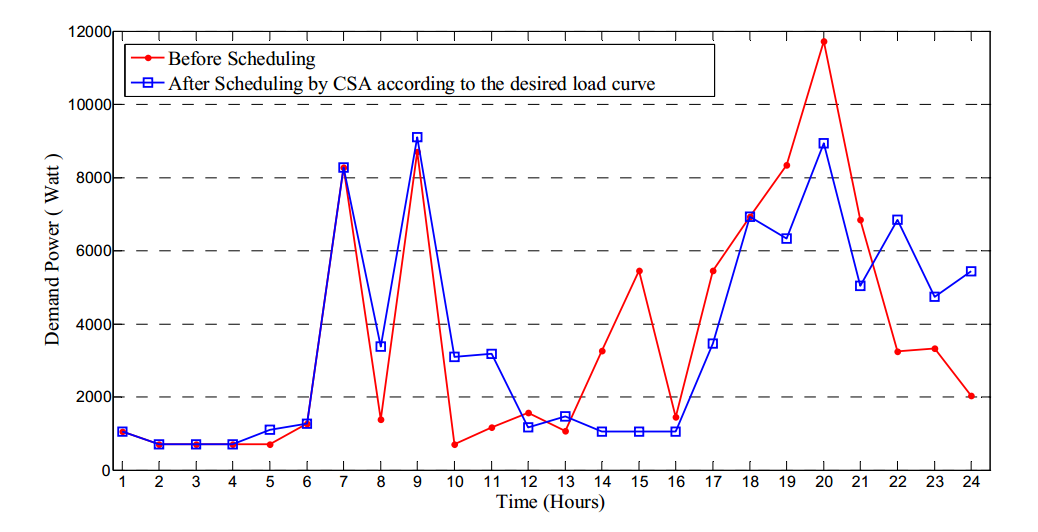
\includegraphics [scale=0.3]{./Figures/t01}
  	\end{center}
  \end{figure}
\end{frame}

\begin{frame}
  \begin{block}{}
   \begin{itemize}
     \item Relatório de estudo de demandas da Empresa de Pesquisa energética EPE.
     \item Projeção de 2016/2026.
       \begin{itemize}
         \item Demanda atual ~ 541 TWH.
         \item Projeção 2050 ~ 1.624 TWH.
       \end{itemize}
   \end{itemize}
  \end{block}
  \begin{figure}[h]
  	\begin{center}
      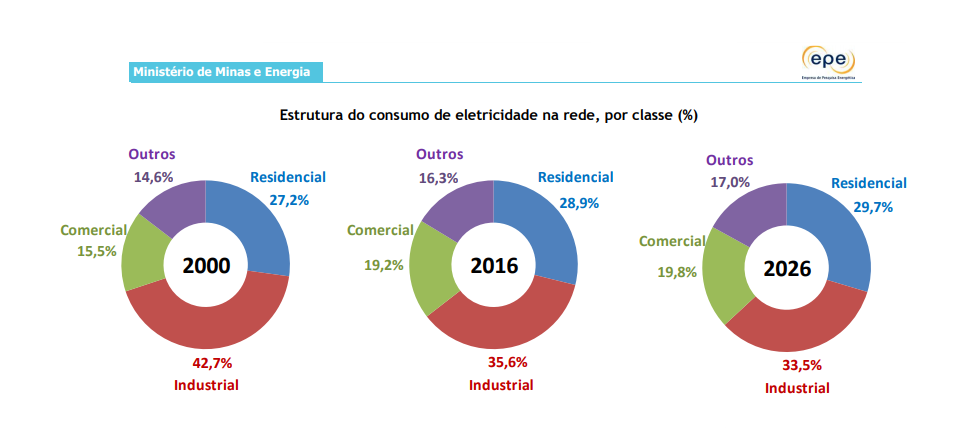
\includegraphics [scale=0.2]{./Figures/t02}
  	\end{center}
  \end{figure}
  \begin{figure}[h]
  	\begin{center}
      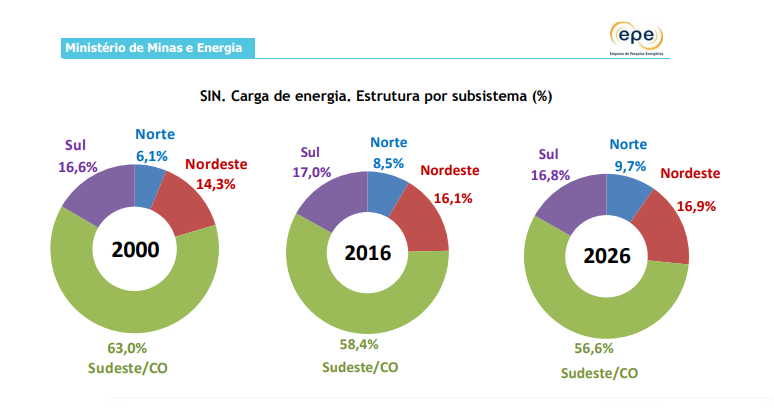
\includegraphics [scale=0.2]{./Figures/t03}
  	\end{center}
  \end{figure}
\end{frame}

\begin{frame}
  \begin{block}{}
   \begin{itemize}
      \item Compensação de Energia Elétrica com as Condições Gerais de
        Fornecimento (Resolução Normativa nº 414/2010).
   \end{itemize}
  \end{block}
  \begin{figure}[h]
  	\begin{center}
      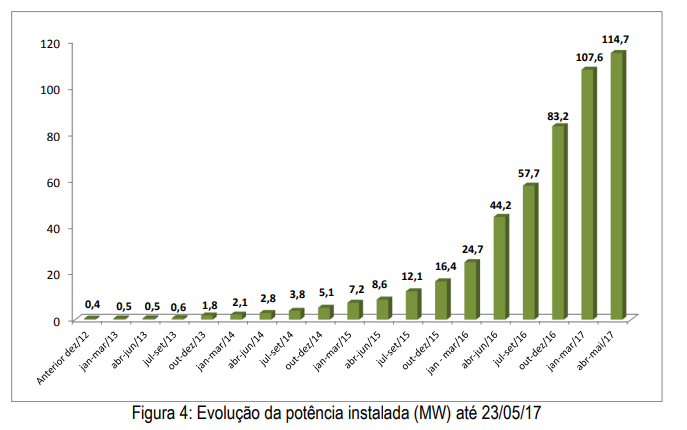
\includegraphics [scale=0.3]{./Figures/t04}
  	\end{center}
  \end{figure}
\end{frame}

\begin{frame}
  \begin{block}{}
   \begin{itemize}
        \item Aumento da quantidades de fontes na rede.
        \item Projeção de crescimento para os próximos anos.
        \item Maior disponibilidade de energia.
   \end{itemize}
  \end{block}
	\begin{figure}[!htb]
		\centering
		\subfloat[]{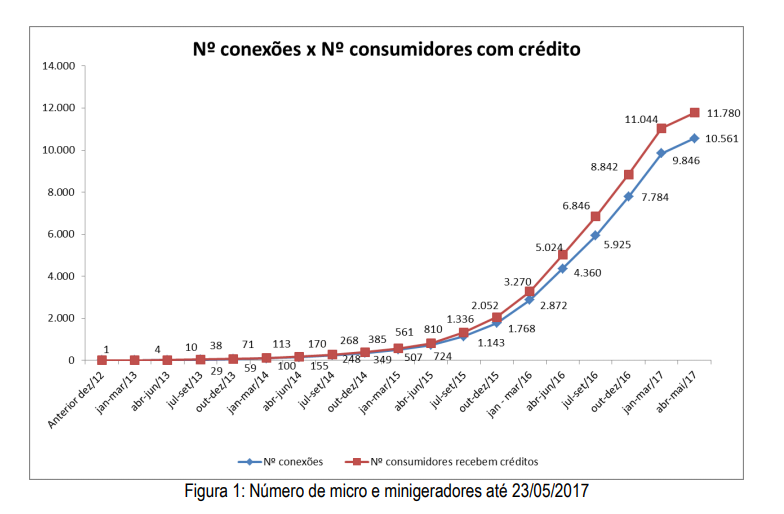
\includegraphics[height=3.4cm]{./Figures/t05}}
		\quad %espaco separador
		\subfloat[]{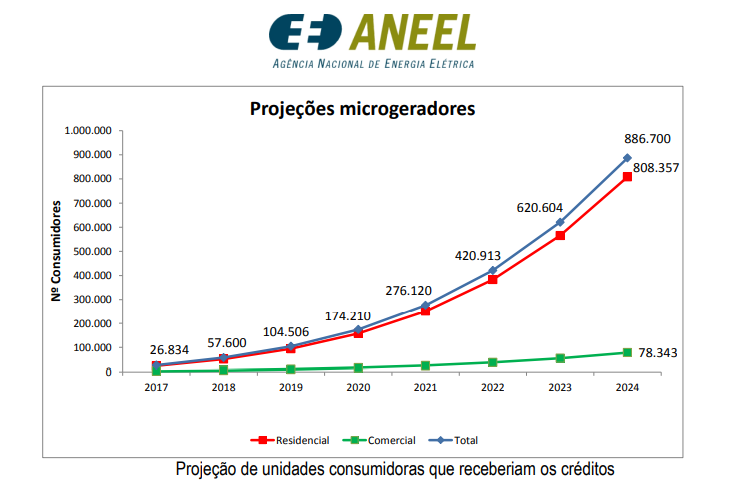
\includegraphics[height=3.4cm]{./Figures/t06}}
	\end{figure}
\end{frame}

\begin{frame}
  \begin{block}{}
   \begin{itemize}
     \item Fonte solar responde por 70\% e a eólica por 9\%.
   \end{itemize}
  \end{block}
	\begin{figure}[!htb]
		\centering
		\subfloat[]{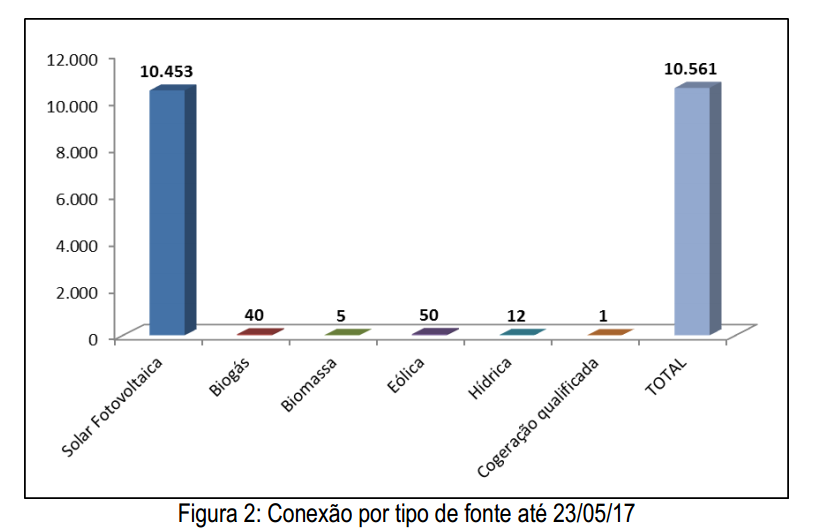
\includegraphics[height=3.4cm]{./Figures/t07}}
		\quad %espaco separador
		\subfloat[]{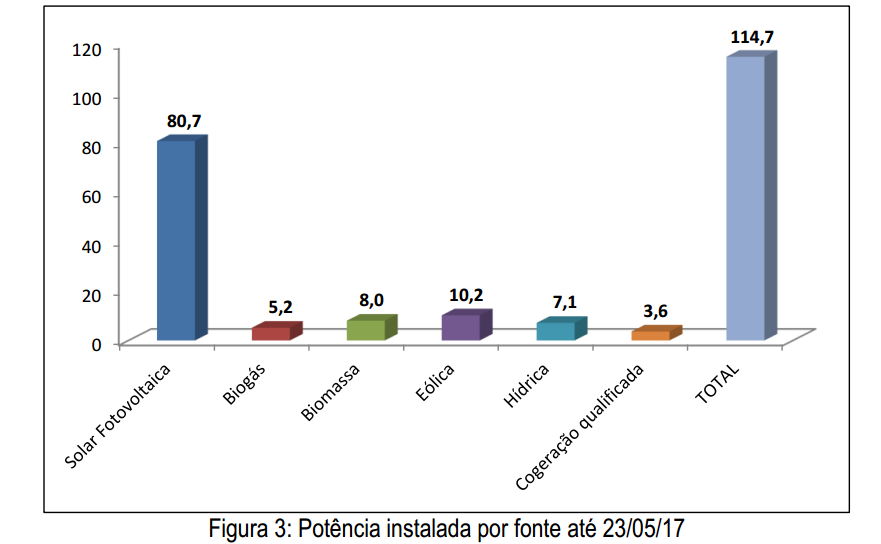
\includegraphics[height=3.4cm]{./Figures/t08}}
	\end{figure}
\end{frame}

\begin{frame}
  \begin{block}{}
   \begin{itemize}
     \item Deslocamento de carga par a horários com menor demanda e máxima
       geração local.
     \item Nota Técnica n 0056/2017-SRD/ANEEL
   \end{itemize}
  \end{block}
  \begin{figure}[h]
  	\begin{center}
      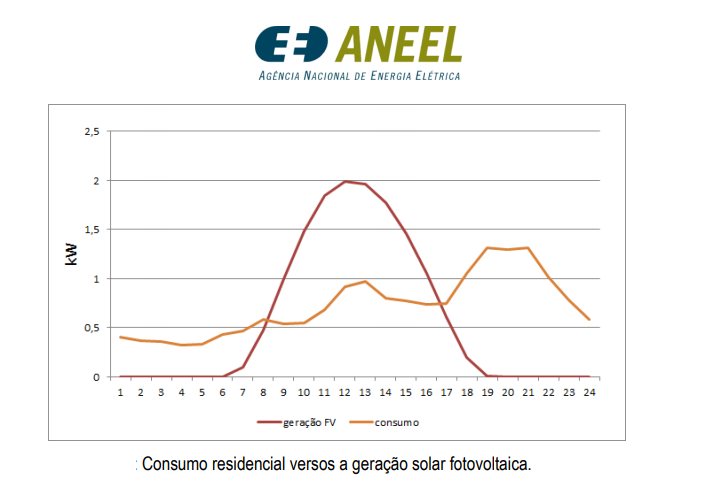
\includegraphics [scale=0.3]{./Figures/t09}
  	\end{center}
  \end{figure}
\end{frame}

\begin{frame}
  \begin{block}{Fundo do Clima BNDES}
   \begin{itemize}
     \item Financiamento à aquisição e à produção de máquinas e equipamentos
      com maiores índices de eficiência energética.
   \end{itemize}
  \end{block}
  \begin{figure}[h]
  	\begin{center}
      
\includegraphics [scale=0.3]{./Figures/t10}
  	\end{center}
  \end{figure}
\end{frame}

\begin{frame}
  \begin{block}{Conclusões}
   \begin{itemize}
     \item Os resultados diretos/indiretos sobre a realocação ótima de cargas
       em relação a demanda.
       \begin{itemize}
         \item Redução de custos gerais com energia.
         \item Reajuste tarifário com menor impacto \%.
         \item Melhores níveis de tensão.
         \item Aumento do número de fonte renováveis grade de geração.
         \item Redução de custos para companhias de energia elétrica com
           expansão de redes.
         \item Melhor eficiência sobre o carregamento de transformadores.
       \end{itemize}
   \end{itemize}
  \end{block}
\end{frame}

%\begin{frame}
%  \begin{figure}[h]
%  	\begin{center}
%      \includegraphics [scale=0.3]{./Figures/Device-Estimates}
%     % \caption {Estimativa de dispositivos conectados à Internet.}
%  		%\label{fig:arq-imuno}
%  	\end{center}
%  \end{figure}
%\end{frame}

%\begin{frame}{Redes de Acesso}
%	\begin{figure}[!htb]
%		\centering
%		\subfloat[DSL]{
%			\includegraphics[height=3.5cm]{./Figures/DSLaccess}
%			\label{figdroopy}}
%		\quad %espaco separador
%		\subfloat[Cable]{
%			\includegraphics[height=3.5cm]{./Figures/CableAccess}
%			\label{figsnoop}}
%		%\caption{Subfiguras}
%		%\label{fig01}
%	\end{figure}
%\end{frame}

%\begin{frame}[fragile]
%\scriptsize
%\begin{verbatim}
%\end{verbatim}
%\end{frame}

%\begin{frame}{\textit{Socket Programming with TCP}}
%\scriptsize
%\lstinputlisting[language=Python, caption={TCP Server.}]{./code/upperServer/TCPserver.py}
%\end{frame}



%\section{Referências}
%\frame{\tableofcontents[currentsection]}

\begin{frame}[allowframebreaks]{Referências}
% \bibliography{../referencias}

\begin{thebibliography}{10}
		\bibitem{smartgrid-cso}[1]
			"Scheduling of domestic shiftable loads via Cuckoo Search optimization
      algorithm."
      \newblock Cakmak, Recep, and Ismail H
      \newblock Smart Grid Congress and Fair (ICSG), 2016 4th International
      Istanbul. IEEE, 2016
		%\bibitem{class}[2]
		%	Author name
		%	\newblock Title.
		%	\newblock Conference, 2018.
\end{thebibliography}
\end{frame}

\begin{frame}{Dúvidas?}
  \begin{figure}[h]
  	\begin{center}
      
\includegraphics [scale=0.4]{./Figures/duvida}
      %\caption {Modelagem Geral do Sistema Imuno.}
  		%\label{fig:arq-imuno}
  	\end{center}
  \end{figure}
\end{frame}

%\begin{frame}
%	\begin{block}{}
%		\begin{center}
%			\textbf{Obrigado pela aten\c{c}\~{a}o!}
%		\end{center}
%	\end{block}
%	\begin{itemize}
%  		\item andresp@lasca.ic.unicamp.br
%  	\end{itemize}
%	\vspace{2cm}
%\end{frame}


\end{document}
